\chapter{Introduction}

\todo{Brief introduction, add more stuff...}
This project is done in order to design a new architecture of a existing recording system developed at SDU.  The existing recording system cannot be used in all usescases, as it has limitations in the existing design. 

\section{Use Cases}
The use cases have been found by talking to biologists that use sound recordings to do experiments with animals, and with the developers of the existing system. The list of use cases is not exhaustive but includes the most relevant use cases with unique requirements.
\todo{Describe which are present, which are future}

\subsection{Existing Use Cases}
The following use cases have been used or is currently being used.

\subsubsection{Bats}
The biologists at SDU do experiments with bats to gain knowledge about how bats use their echolocation, where bats live, and where they live in the nature.
Some of the experiments are conducted as described in section \ref{sec:usecase:porpoise} with porpoises. Instead of doing the experiments in water, they are conducted in a batcage shown in figure \ref{fig:usecase:batcage}. When the bats fly towards the bait, the biologist can create a recording using the trigger mechanism, as described in \ref{sec:usecase:triggerrecording}.

\begin{figure}[!h]
    \centering
    \begin{subfigure}[b]{0.45\textwidth}
        \includegraphics[width=\textwidth]{figures/batcage_cross}
        \caption{Figure of batcage with existing system's microphone mount}
        \label{fig:gull}
    \end{subfigure}
    ~ %add desired spacing between images, e. g. ~, \quad, \qquad, \hfill etc. 
    %(or a blank line to force the subfigure onto a new line)
    \begin{subfigure}[b]{0.45\textwidth}
        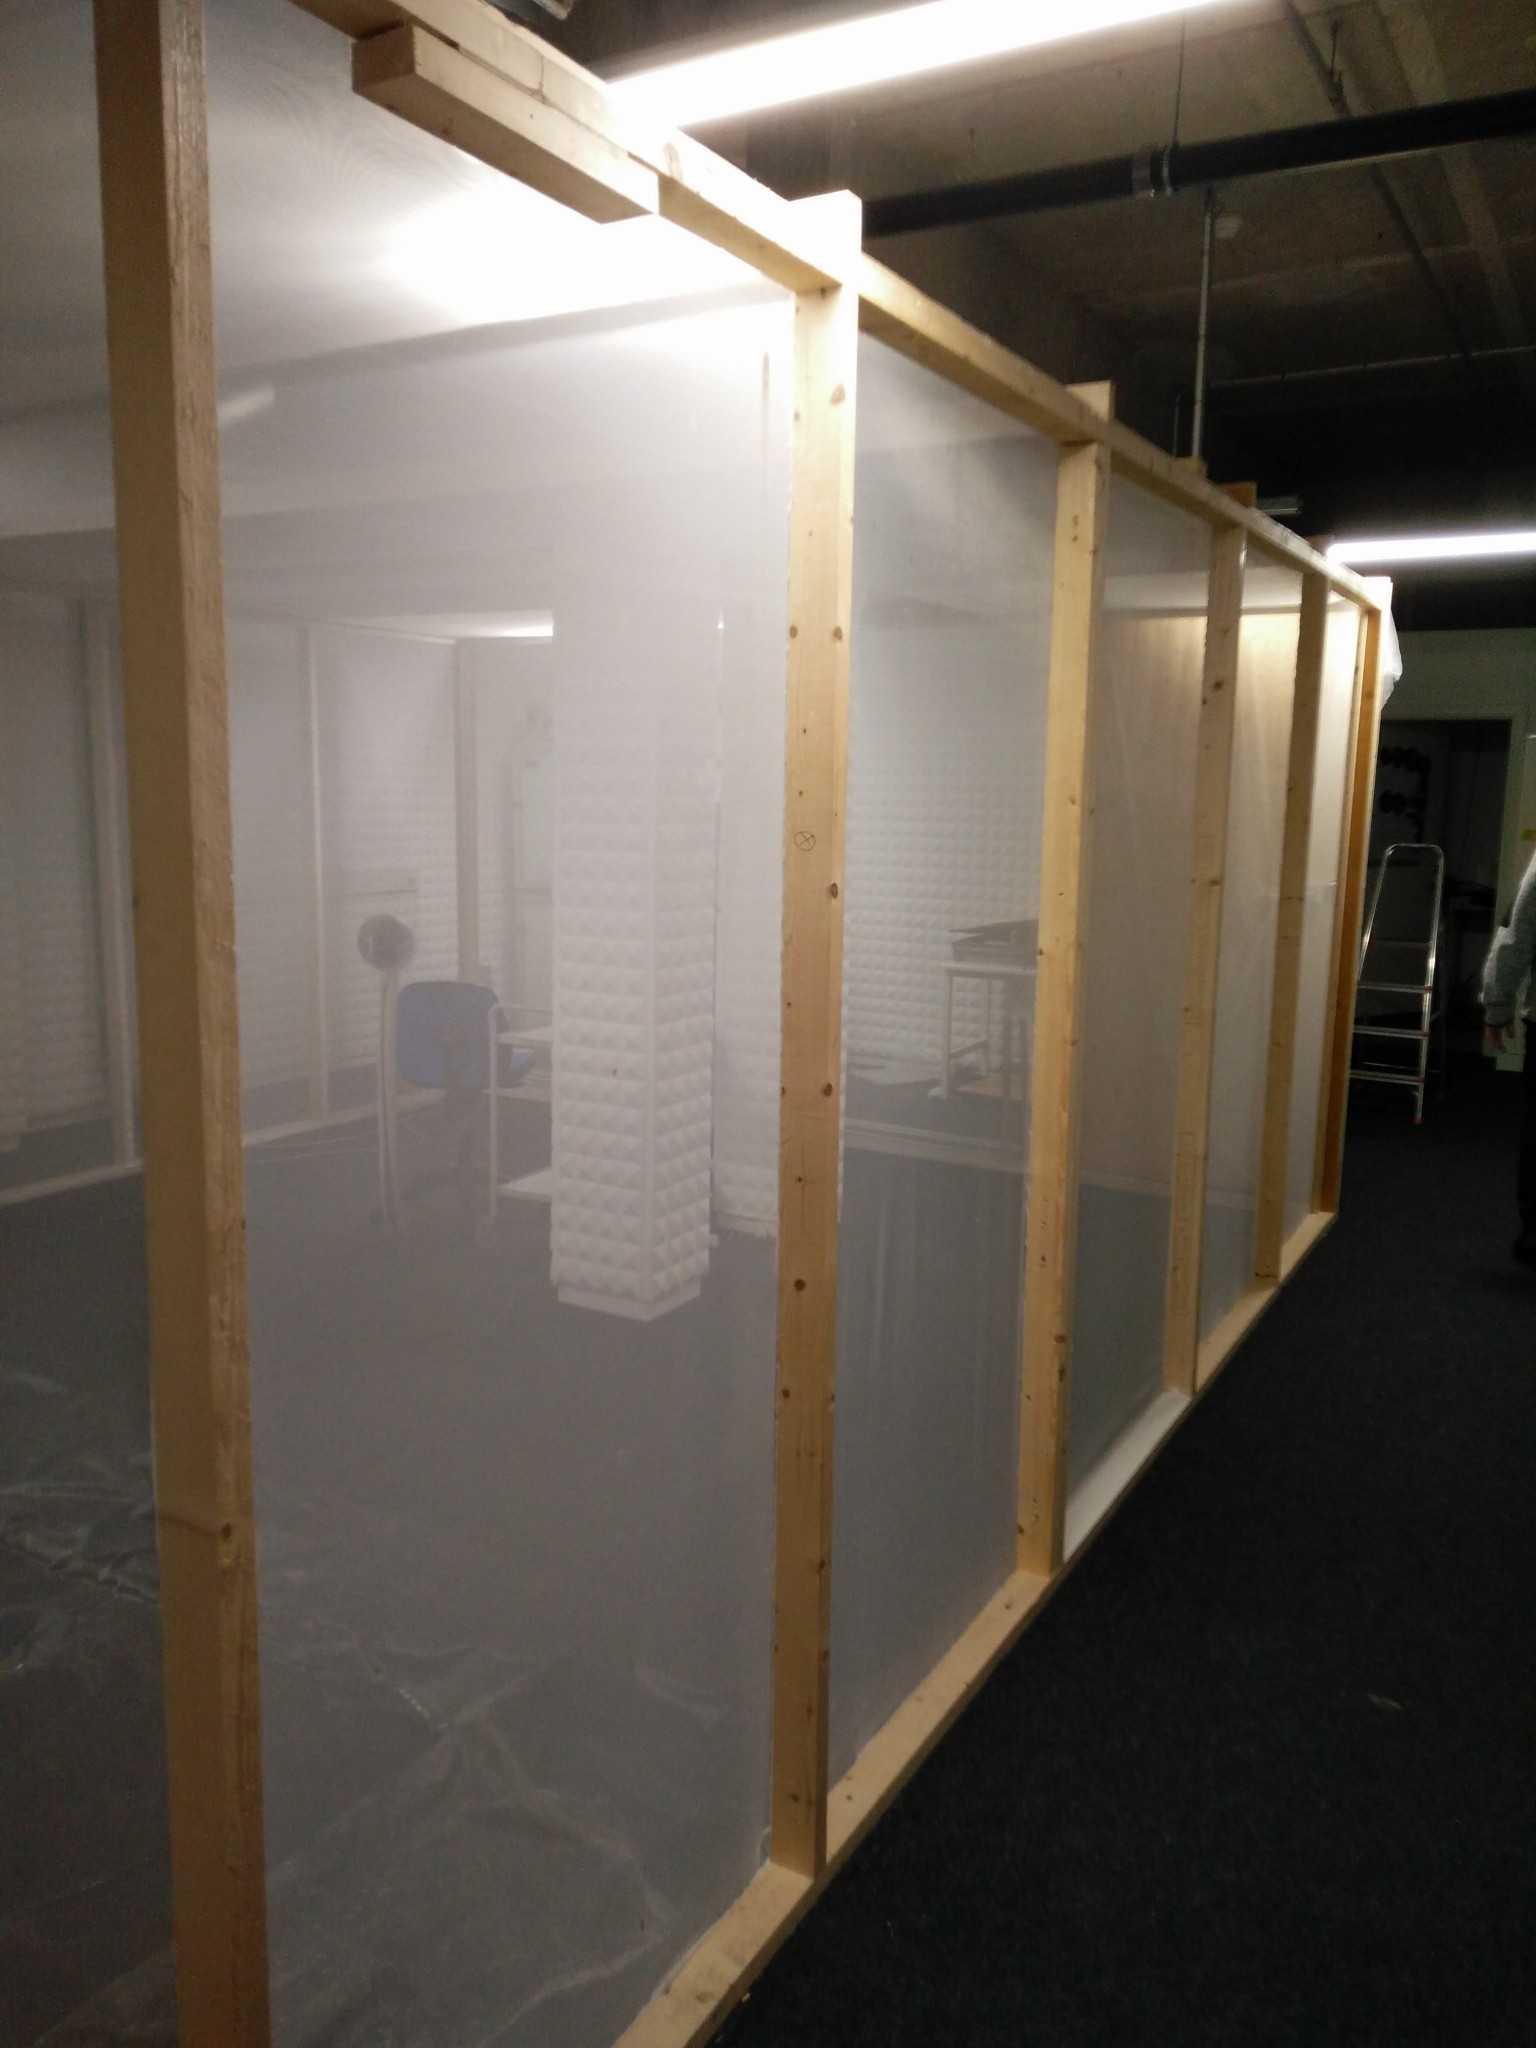
\includegraphics[width=\textwidth]{figures/batcage}
        \caption{Figure of the opposite end of the batcage}
        \label{fig:mouse}
    \end{subfigure}
    \caption{Pictures of batcage}\label{fig:usecase:batcage}
\end{figure}

Another set of experiments were conducted in Panama. 8 microphones are mounted in a tree, in order to investigate which bat species live in the forest. As the microphones and the batbox is mounted in a forest, the batbox is running on battery. Due to the location of the recording system in a forest, it's cumbersome to get physical access to the system, to do maintenance like replacing battery, hard drives etc. The system therefore do periodically \textit{short recordings} as described in section \ref{sec:usecase:shortrecordings}. 

A third experiment is done in Odense where the new hospital will be built.
%The idea is to investigate how the new hospital will affect the bats living in the area.
The idea is to put up N batboxes, each with 8 microphones in the area where the hospital will be build to get more knowledge about the bats that live in the area. During  construction of the hospital and after the hospital has been built, the biologists want to know if the behaviour of bats have changed. The system should only do recordings in the night hours as bats are not active during daytime. This is described in section \ref{sec:usecase:shortrecordings}.

The biologists also have interest in mounting a batbox with a microphone on drones. An experiment is to manually steer a drone near a group of flying bats, to gain knowledge about how bats behave in the air, which species fly at different heights etc. This should in the future be automated such that two drones, each with 4 microphones and a batbox can point in the direction of the group of bats. In order to maintain the heading, the drones should emulate being a bat by emitting ultrasonic sounds which is then recorded by the microphones. The trigger recordings must be minimum 30 ms. To do this, processing of the recordings must be done online, as described in section \ref{sec:usecase:online}.
These experiments require long recordings as described in section \ref{sec:usecase:longrecording} in order to record while the drone is in the air and triggered-recording as described in section \ref{sec:usercase:longrecording} to listen for ultrasonic replies emitted by the drone.

\subsubsection{Frogs}
Biologists also have interest in recording frogs, in order to learn more about their vocalization capabilities. Frogs use advanced techniques to synchronize with other frogs, so they alternate vocalization to increase their change of being heard by females frogs. Furthermore they use techniques where they do vocalizing near a bigger male frog to amplify their vocalization to, as before, increase their change of getting hear by female frogs. Figure \ref{fig:usecase:frogs} shows an illustration of frogs vocalizing around a lake. Experiments are usually conducted by mounting 8 microphones and 1 batbox close to a lake. The system is running on battery and requires recording to be done in predefined period of time during daytime. This system requires short recordings as described in section \ref{sec:usecase:shortrecording}

\begin{figure}[H]
	\centering
	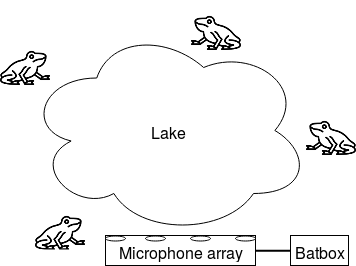
\includegraphics[width=0.6\textwidth]{figures/usecases_frogs}
	\caption{Figure of frogs sitting around a lake while the batbox is recording with 4 microphones} \label{fig:usecase:frogs}
\end{figure}

\myparagraph{Drones} \label{sec:usecase:drone}
Drones are used to take pictures of the ocean, to see where porpoises are living.
%Drones will also be used in the future to investigate where salmon\todo{not salmon but?} breed in Denmark, as this is not known.
Since the drone is hovering over the ocean, the biologists want to lower a hydrophone into the water from the drone, to listen to porpoises and other sea activity. This is sketched in figure \ref{fig:usecase:drone}.

\begin{figure}[h!]
	\centering
	
\includegraphics[width=0.4\textwidth]{figures/usecase_drone}
	\caption{Figure of the drone with a hydrophone hanging form the drone. The hydrophone is lowered into water to listen to sea animals}\label{fig:usecase:drone}
\end{figure}

In the beginning the system will only use one hydrophone, but in the future the might use more to do ecolocation to get the position of the sound source in the ocean.
The system will do short recordings as described in section \ref{sec:usecase:shortrecording}, as they only want to record if the drone detects any activity in the ocean.

\subsubsection{Zebra Finches}
Biologists use Zebra Finches for investigating vocalization, as the Zebra finch has a stereotypical sound, are easy to breed and has a well-defined song-learning process. Especially the tutoring session between a young bird and its father has been investigated thoroughly. In an experiment, a teleconference system for birds has been build. The two birds are physically isolated in boxes, but can communicate via cameras, screens, microphones and speakers. One of the goals of this project is to do much of the audio and video processing online. One batbox has been used, where 1 microphone is placed in each of the two boxes.\citep{larsen2016system}
Figure \ref{fig:usecases:zebra:overview} shows the conceptual design of the experiment:

\begin{figure}[h!]
	\centering
	
\includegraphics[width=0.6\textwidth]{figures/zebrafinches_experiment1.png}
	\caption{Pictures of experiment with zebra finches where only microphones, batbox and speakers are depicted}\label{fig:usecases:zebra:overview}
\end{figure}
It should be noted, that only two microphones are in use in this system.
As the system is designed to replay tutoring sessions from previous experiments, it is required that the system can replay recordings.
The system uses long recordings as described in section \ref{sec:usecase:longrecording}.


\subsection{Future Use Cases}
The following use cases have not been conducted yet, but will be conducted in the near future.

\subsubsection{Porpoise}
The biology department in Kerteminde conducts experiments with porpoises in order to gain an understanding of how their ultrasonic echolocation works.
%The U.S. Navy currently use dolphins to locate mines as they are better than human engineered solutions \foodnote{https://www.dolphins-world.com/dolphins-in-the-military/}. The general testsetup is depicted in figure \ref{usecase:porpoise_experiment1}.
\begin{figure}[!h]
    \centering
	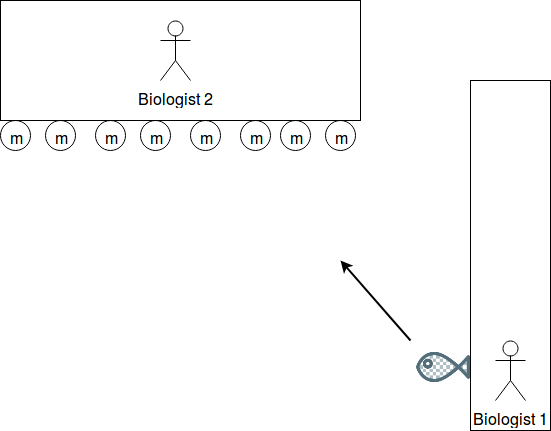
\includegraphics[width=\textwidth]{figures/porpoise_experiment1}
	\caption{Figure of test setup of porpoise's echolocation. The two boxes indicate piers, each with a biologist standing. On pier 2, 8 hydrophones are mounted.}\label{usecase:porpoise_experiment1}
\end{figure}


Figure \ref{usecase:porpoise_experiment1} shows a porpoise swimming in a basin close to \textit{Biologist 1}.
When \textit{Biologist 2} throws bait in the basin, the porpoise will swim towards the bait while emitting high frequency, narrow band clicks, in order to swim in the direction of the bait. A porpoise emits clicks at a frequency of $\approx$ 130 khz.
Since 8 microphones are mounted near the bait on piers 2, the recording system is able to record the clicks emitted by the porpoise. This experiment exists in different variations where, for instance, different materials are mounted between the bait and the porpoise that tamper with the porpoise's clicks and hearing. The experiments are conducted using one batbox with 8 hydrophones.

These experiments use \textit{Trigger recordings} and \textit{Long recordings} as described in section \ref{sec:usecase:triggerrecording} and \ref{sec:usecase:longrecording} respectively.

\subsubsection{Live Underwater Laboratorium}
The biologists in Kerteminde have an ongoing project where they want to enlighten students in folkeskoler and efterskoler about nature under water. They want to to stream live sound from the ocean in Kerteminde. Furthermore, they want to show live measurements of salinity, pH and temperature of the ocean to the students.
This system will also be used to investigate how ferries etc. affect the lives of the animals living in the ocean. Biologists usually do experiments with fish in captivity, but they know very little about the life in the ocean outside their window. Ideally the biologists wants to get an notification when a fish or animal of interest is located in the ocean around Fyn. This usually requires \textit{long recordings} as described in section \ref{sec:usecase:longrecording}.




\subsection{Recording Types} \label{sec:usecase:recordingtypes}
\begin{figure}[h!]
    \centering
    \begin{subfigure}[b]{0.3\textwidth}
        
\includegraphics[width=\textwidth]{figures/recording_trigger.png}
        \caption{Trigger recording illustrated}
        \label{fig:usecase:triggerrecording}
    \end{subfigure}
    ~ %add desired spacing between images, e. g. ~, \quad, \qquad, \hfill etc. 
      %(or a blank line to force the subfigure onto a new line)
    \begin{subfigure}[b]{0.3\textwidth}
        
\includegraphics[width=\textwidth]{figures/recording_long.png}
        \caption{Long recording illustrated}
        \label{fig:usecase:longrecording}
    \end{subfigure}
    ~ %add desired spacing between images, e. g. ~, \quad, \qquad, \hfill etc. 
    %(or a blank line to force the subfigure onto a new line)
    \begin{subfigure}[b]{0.3\textwidth}
        
\includegraphics[width=\textwidth]{figures/recording_short.png}
        \caption{Short recording illustrated}
        \label{fig:usecase:shortrecording}
    \end{subfigure}
    \caption{Illustration of the three types of recordings}\label{fig:usecase:recordingtypes}
\end{figure}
\subsubsection{Long Recordings}\label{sec:usecase:longrecording}
Long recordings are used in experiments where it is required to do continuous recordings for, theoretically, indefinitely. Long recordings are used where either storage is always available or the local attached storage can be replaced when out of space. Long recordings  require external power is connected the system, and that it is not running on battery. A long recording is shown in figure \ref{sec:usecase:longrecording}.

\subsubsection{Trigger Recordings}\label{sec:usecase:triggerrecording}
Trigger recordings are used in experiments where it potentially takes a long time before the event of interest is happening. By using a trigger recording, the recording can be triggered after the event has happened, but where the event is saved in the recording. In figure \ref{fig:usecase:triggerrecording} two microphones are depicted with respect to time. When the system receives a trigger, it will export the recording to the the biologist, starting at $trig-pre$ to $trig+post$. The duration of the recording will therefore be $pre+post$. The trigger is usually received by a press on a button.

\subsubsection{Short Recordings}\label{sec:usecase:shortrecording}
Short recordings are used when the storage is limited or the batbox is not always powered up due to power constrains such as the batbox is running on battery. The start of the recording and duration must be specified such that the biologists can key in when the recordings should be conducted.
A short recording is depicted in figure \ref{fig:usecase:shortrecording}.


\subsection{Data Analysis} \label{sec:dataanalysis}
%Analysis of recordings are usually done in one of three ways: online, offline or as batch processing.
The goal of data analysis is to extract knowledge from the recordings. Extracted knowledge from recordings are usually referred to as Events, as they describe what happens at at given moment in time, for how long time it happens and then some associated data explaining what exactly happens.
By talking with biologists, the analysis of recording has been split into three groups: online, offline and batch processing. 

\myparagraph{Online}\label{sec:usecase:online}
Online processing is when the processing is happening while the experiment is conducted. This implies that recordings and results can be used in the experiment such as in the \textit{Zebra Finches experiment}, where tampering with data online is important. Recordings can be saved, but is not required to. This also allows systems to only save the result of the processing meaning much less storage is needed.

\myparagraph{Offline}
Offline analysis is used in most use cases where the recordings are saved to local storage. The processing of the recordings can be done when the storage is brought back from the test location. When the recordings are replayed, it should emulate the online recordings.
It should be possible to replay the same recording multiple times, where it can be chosen when the replay should happen from. Furthermore it must be possible to specify the duration of the replay. It is required the replaying has a granularity of 1 second. In cases where multiple microphones or hydrophones together with sensors are recorded, it should be possible to specify which microphone or sensor to replay

\myparagraph{Batch Processing}
Batch processing is also happening offline, but in this case the recordings are exported as  files, which can be used on a supercomputer such as Abacus. The different between offline and Batch Processing is the fact, that in offline-analysis, the format of the recordings is raw and requires pre-processing.\\

Table \ref{tab:recordingtypes:summarize} summarizes how the different use cases use the recording types.

% Please add the following required packages to your document preamble:
% \usepackage{graphicx}
\begin{table}[!h]
\centering
\resizebox{\textwidth}{!}{%
\begin{tabular}{|l|l|l|}
\hline
\textbf{Use Case} & \textbf{Recording Type} & \textbf{Analysis}    \\ \hline
Porpoises         & Trigger/Long            & Online               \\ \hline
Bats              & Trigger/Long/Short      & Online/Offline/Batch \\ \hline
Frogs             & Short                   & Online/Offline/Batch \\ \hline
Zebra Finches     & Long                    & Online               \\ \hline
\end{tabular}%
}
\caption{Table that summarizes the uses cases with the type of recording and analysis they use}
\label{tab:recordingtypes:summarize}
\end{table}

\section{Current System Architecture}

% The system supports sampling of 312.5 khz on each channel where the present version of the hardware has 8 channels. 
A recording system has been developed by John Hallam \& T{\'o}rur Andreassen \citep{andreassen2013ultrasonic} named \ac{MCLURS}, which is used on most of the usescases list in section \ref{sec:usecase}. The hardware of MCLURS is described in section \ref{sec:currentsystem:hw}. 
However due to MCLURS's design, it has some limitations which cannot be bypassed without redesigning the overall architecture. Limitations of the existing system are described in section \ref{sec:existingsystem:limitations}.\\


MCLURS is illustrated in figure \ref{fig:existingsystem:overview}. The yellow and blue boxes are hardware and software components respectively.


\begin{figure}[h!]
	\centering
	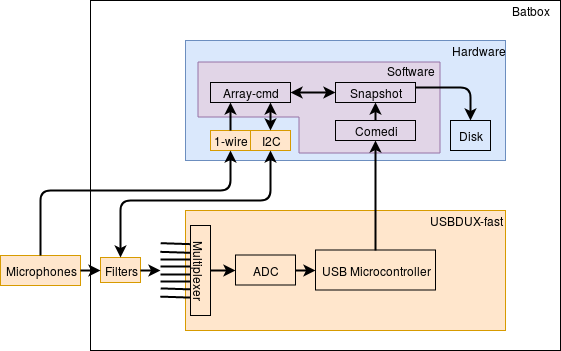
\includegraphics[width=1\textwidth]{figures/existing-system-overview.png} 
	\caption{Overview of existing system. Yellow boxes indicate hardware and blue boxes are software components.}\label{fig:existingsystem:overview}
\end{figure}

\subsection{Hardware}
The hardware used in MCLURS is shown in figure \ref{fig:existingsystem:hardware}.

\begin{figure}
    \centering
    \begin{subfigure}[b]{0.45\textwidth}
        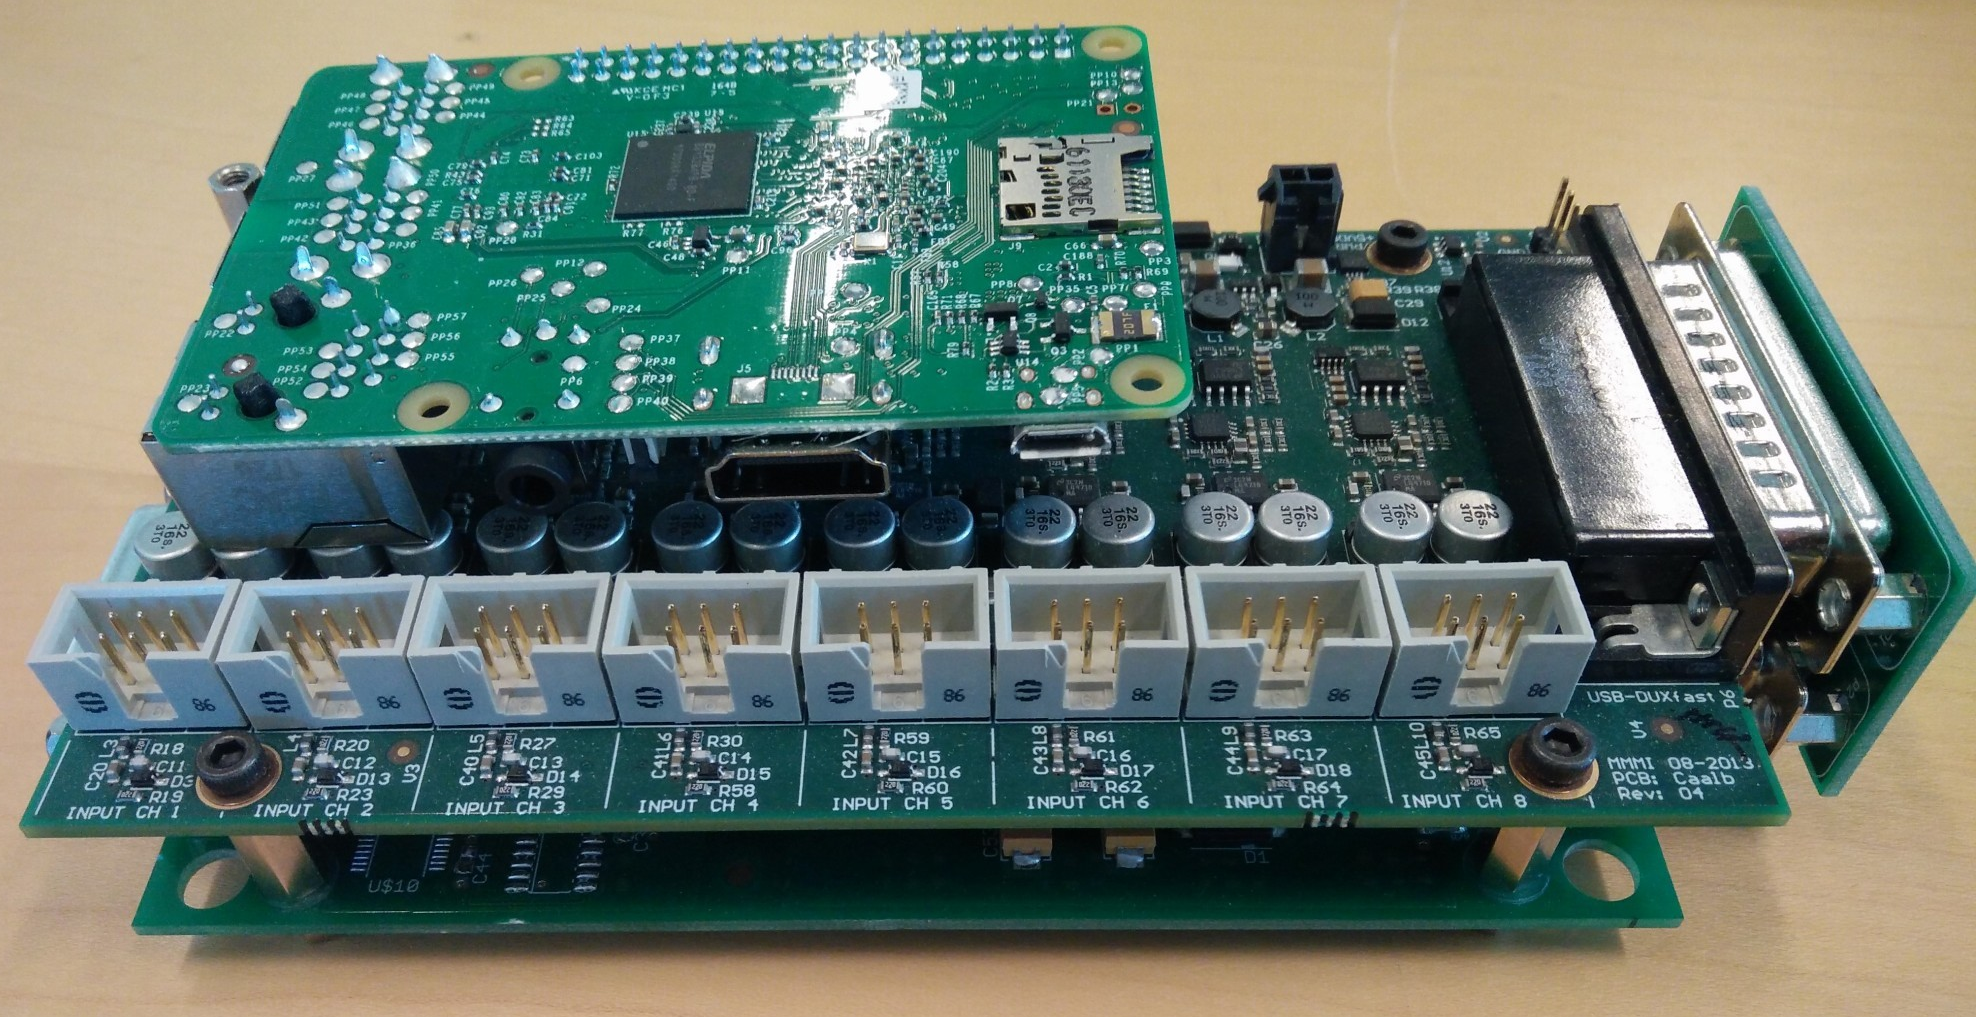
\includegraphics[width=\textwidth]{figures/batbox}
        \caption{Figure showing the three PCBs. The PCBs are: RPI, Analog PCB and USBDUX from top to buttom}
        \label{fig:gull}
    \end{subfigure}
    ~ %add desired spacing between images, e. g. ~, \quad, \qquad, \hfill etc. 
    %(or a blank line to force the subfigure onto a new line)
    \begin{subfigure}[b]{0.45\textwidth}
        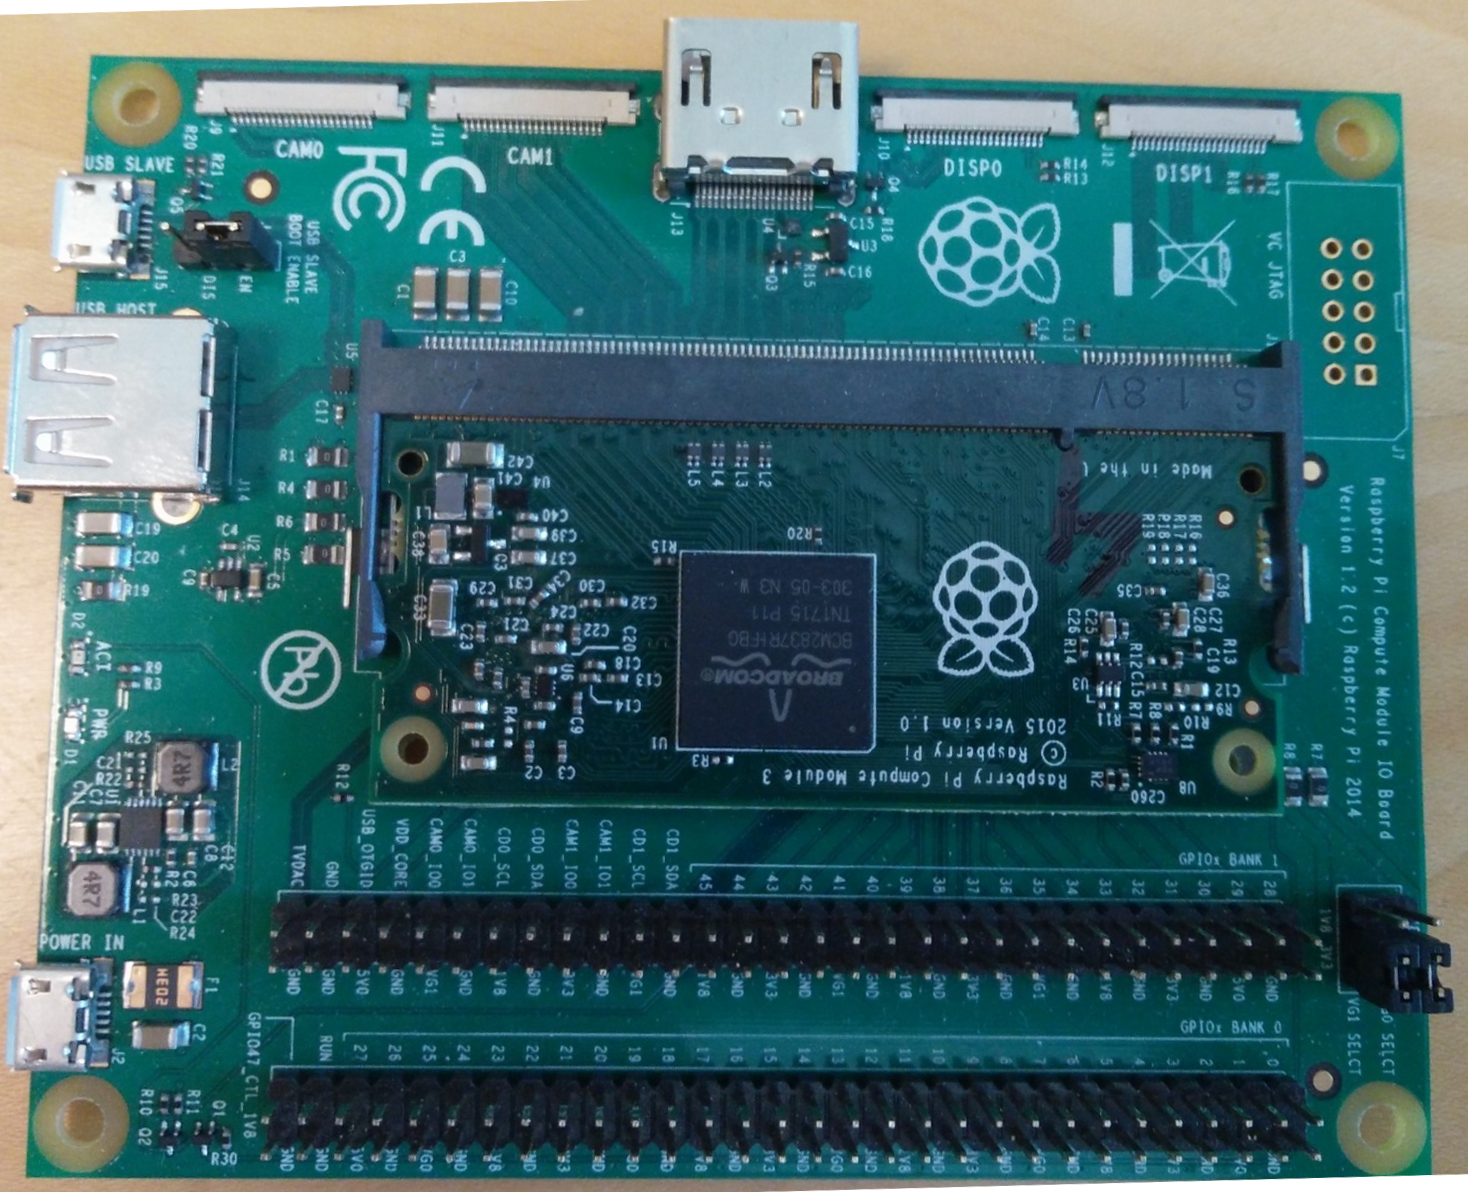
\includegraphics[width=\textwidth]{figures/drone_pcb}
        \caption{Figure showing the drone-pcb. The PCB in in the middle is a \textit{RPI compute module}}
        \label{fig:mouse}
    \end{subfigure}
    \caption{Images of the two MCLURS hardware versions.}\label{fig:intro:batbox}
\end{figure}

The hardware consists of 3 PCBs, each listed and described below:
\begin{enumerate}
	\item \textbf{Raspberry Pi} The Raspberry Pi runs the software described in section \ref{sec:existingsystem:software}. It interfaces the Analog PCB through GPIO headers on the RPI, and the USBDUX through USB.
	
	\item \textbf{USBdux-fast} The USBdux-fast board is responsible for sampling the 8 channels. The USBDUX-fast has an ADS807 ADC, which is a single channel ADC capable of sampling at 53Mhz.\citep{ADC:ADS807}. The USBdux-fast is connected to the RPI via a USB 2.0 port.
Since the system has 8 channels, a multiplexer is placed in front of the ADC, that cycles through the 8 channel inputs.
The ADC and multiplexer are controlled by the onboard peripheral USB micocontroller(cy7c68013a) which instructs the ADC when to do sampling and the multiplexer to select a channel. Due to internal limitations of the USBdux-fast, it's sample frequency of a single channel is 376 khz, which equals 3.008 mhz in total for all 8 channels. As each sample is 16 bits(2 bytes), this equals a total bandwidth of 6 mb/sec, when the ADC is sampling at full speed. The microcontroller is running a firmware as explained in section \ref{sec:existingsystem:software:kernelmodule}.
	
	\item \textbf{Analog PCB} The Analog PCB is responsible for the 1W-interface to the microphones\todo{intorducte 1W somewhere}, the RTC, setting gain, filters, LEDs and proving power for the hardware
\end{enumerate}

Four versions of the hardware exist, however; changes from version 1 to version2B were bugfixes and the addition of a switch to control the filters. The two relevant versions are \textit{Version 2B} and droneboard, as shown in figure \ref{fig:existingsystem:hardware:2B} and \ref{fig:existingsystem:hardware:droneboard} respectively.

\begin{itemize}
	\item \textbf{Version2B} Is the version used in existing use cases. 

	\item \textbf{Droneboard} Is to be used in use case \ref{sec:usecase:drone}. This PCB is designed to be small and light, as it will be mounted on a drone as payload. The PCB is a merge of the \textit{Analog PCB} and USBDUX-fast, however the ADC has been replaced with a LTC2205CUK\citep{ADC:LTC2205} that is 16 bits and has a maximum sample frequency of 65 mhz. Except for the size of a sample and frequency, the interface from the software perspective remains the same as Version2B. To further reduce the weight, the microphone connectors are removed, meaning no EEPROMs are available and thereby no need for the 1W-interfaces on the \textit{Analog PCB}.

In daily speed, a recording box consisting of a RPi, Analog PCB and USBDUX-fast is referred to as a \textit{batbox}.

\end{itemize}
\myparagraph{Microphone}
Microphones connected to the MCLURS system usually have a small PCB built-in into the microphone connector. The PCB contains a DS28E05\citep{EEPROM:DS28E05} 112-byte EEPROM, that allows setting microphone calibration parameters and provides a unique microphone identifier. The microphone is showed in figure \ref{fig:existingsysem:hardware:microhpone}. The built-in PCB also contains circuitry that converts the single-ended output from the internal, actual mirophone into a differential output, in order to reduces the risk of electromagnetic noise in long cables

\begin{figure}[h!]
	\centering
	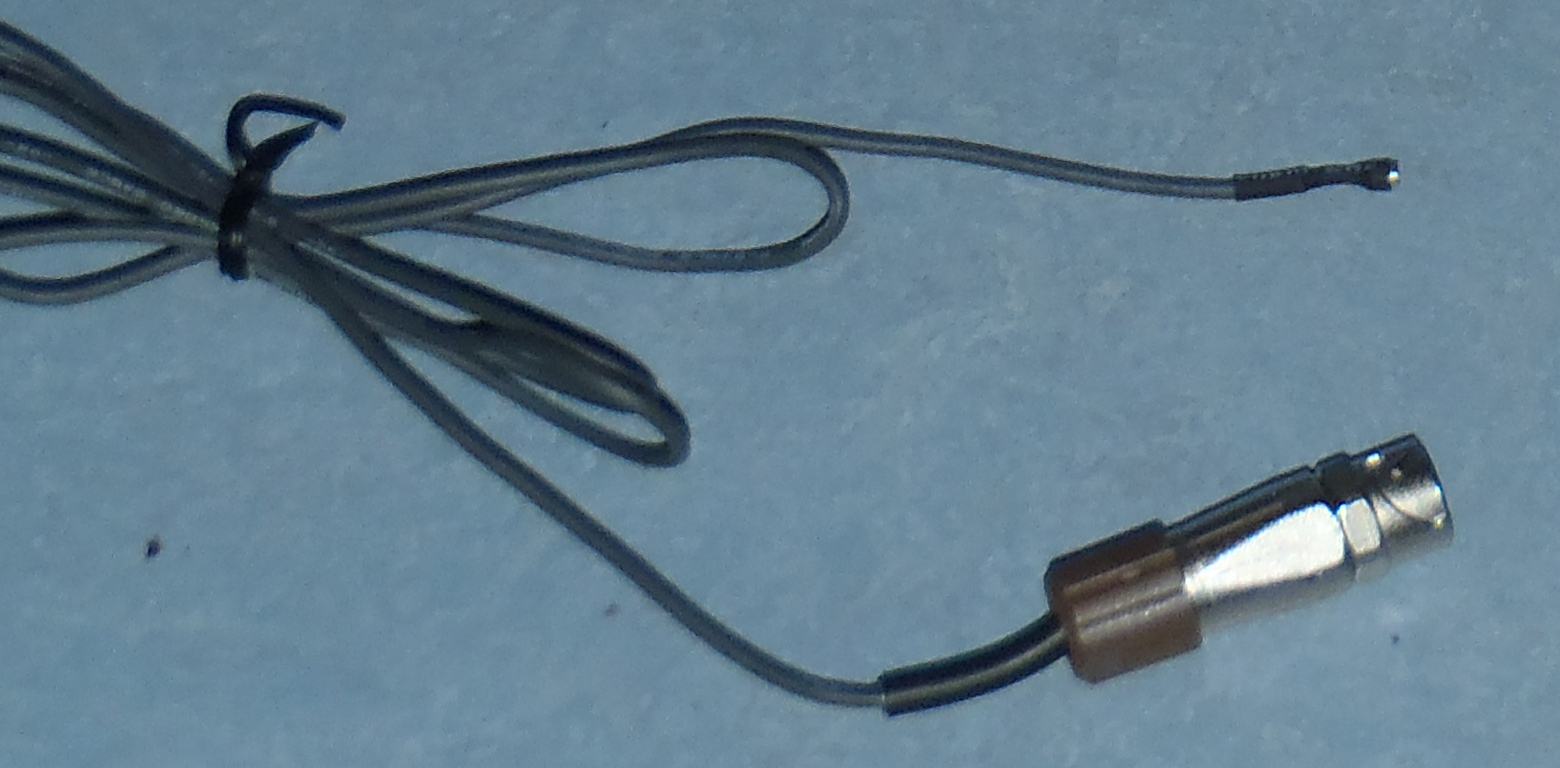
\includegraphics[width=0.5\textwidth]{figures/mclurs_microphone}
\end{figure}
\subsubsection{Software Components} \label{sec:existingsystem:software}
MCLURS consists of a suite of programs that all have a well defined responsibility. Time critical programs are written in C, where non time-critical programs are written in Perl.
The \program{array} program is written in bash, as it is the CLI interface to MCLURS that allows starting recordings etc.

Below is listed the programs in MCLURS:
\begin{itemize}
	\item \textbf{snapchat} is responsible for getting the samples from the usbdux/comedi (see section \ref{sec:existingsystem:software:kernelmodule}) module and writing the samples into files. When \program{snapshot} is initialized, it will record samples, however data is only saved to a circular buffer until it is told to write the buffer into a file. The \program{snapshot} will save part of the circular buffer to a file when it receives a "snap" command. This gives the ability to get a recording, consisting of data from a predefined time before it receives the "snap" command. This makes up the \textit{trigger-recording}. \program{Snapshot} is designed to not miss out samples from the comedi device and thereby not from the ADC. \program{Snapshot} supports long recordings, where it repeats the triggering and saves each trig to a file.
	
	\item \textbf{grab} has overlapping responsibility with \program{snapshot}, however; grab outputs samples to stdout and not by writing to any files. Furthermore, the implementation of the grab node is much more simple, as it has no need to maintain a circular buffer and thereby implements less memory management. If the consuming process blocks its stdin, grab will lose samples. Grab is usually used for short/long-recordings.

	\item  \program{snapchat} is responsible for communicating with \program{snapshot} and/or \program{array-cmd} depending on the use case. \program{Snapchat} takes commands as parameters and forwards them to \program{snapshot} or \program{array-cmd} using ZeroMQ.

	\item \textbf{array-cmd} is responsible for:
	\begin{enumerate}	
		\item Setting up the USBDUX during startup of MCLURS 
		\item Handling GPIO to HMI(Leds)
		\item Saving meta-data about recordings to file
			\begin{itemize}
				\item Sample frequency of each microphone
				\item Gain for each microphone
				\item Unique identifier for each microphone
				\item Enabled filter for each microphone
				\item Creation time of metdatafile
				\item RPi's assigned name
				\item Number of channels
				\item etc.
			\end{itemize}
		
		\item Determining mode of operation
		\item Handling connected microphones.
		\item Being the interface to the system using ZMQ and UDP.
		\item Hardware communication with DAC for filtering over I2C.
	\end{enumerate} 
	
	A flowchart of the functionality of \program{array-cmd} can be found in appendix~\ref{app:array-cmd}. \todo{Add flowchart to appendix}
	
	\item \textbf{trig} instructs the snapshot when to do a snapshot by constructing and sending a “snap” command to either \program{cmd-array} or \program{snapchat}. It can be told to do snaps repeatedly or only once a key has been pressed. \program{Trig} calculates the beginning and end timestamp of the snapshot, where pre and post are given as parameters.
	
	\item \textbf{array} is a script that hides the complexity of the system to ease the interface for the biologists. It is capable of initializing the system, listing connected microphones, setting options on the microphones, starting/stopping recordings etc.

\end{itemize}


Table \ref{tab:existingsystem:software:nodes} lists the different programs and how they are run, in which language and when they are run. Daemon means the program is run under supervison from \textit{runit} and \textit{One-shot} means the program is run when needed.

\begin{table}[h!]
\centering
\resizebox{\textwidth}{!}{%
\begin{tabular}{|l|l|l|}
\hline
\textbf{Node name} & \textbf{Impl. Language} & \textbf{Running mode} \\ \hline
Snapshot           & C                       & Daemon                \\ \hline
Snapchat           & C                       & One-shot              \\ \hline
Grab               & C                       & One-shot              \\ \hline
Trig               & C                       & One-shot              \\ \hline
array-cmd          & Perl                    & Daemon                \\ \hline
array              & Bash                    & One-shot               \\ \hline
\end{tabular}%
}
\caption{My caption}
\label{my-label}
\end{table}


%Hardware - trigger line(master/slave setups)

\myparagraph{Inter-Process Communication}
The interface to the recording system is either UDP or ZMQ using the request/reply-pattern. Communication between the demons and CLI tools is ZMQ. Communication between threads in snapshot is also using ZMQ, however using push-patterns as ZMQ is used to do logging from busy threads.

\myparagraph{Startup and Supervision}
All daemons are run under supervision from the debian runit package. The runit package is both responsible for starting the nodes during startup, but also to keep the nodes running in case one of them crashes. Since runit does not provide any control of the order of startup, some fiddling has been made in order to start the snapshot and array-cmd in the correct order.  \todo{Add more zmq, push/pull see notes from John}


\myparagraph{Kernel module} \label{sec:existingsystem:software:kernelmodule}\todo{Describe how usbdux communicates with snapshot/grab through comedi}

\begin{figure}[h!]
	\centering
	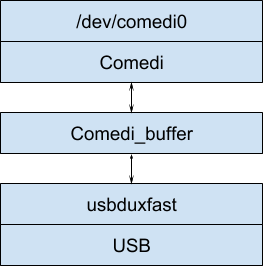
\includegraphics[width=0.4\textwidth]{figures/mclurs_comedi}
\end{figure}

\myparagraph{Software Components} \label{sc:existingsystem:setup}
The MCLURS components described above, can be put together in different ways depending on the use case. Figure \ref{fig:mclurs:grab} and \ref{fig:mclurs:snapshot} shows how the user interacts with the system, what is running on the \ac{RPI} and how it communicates with the hardware. In figure \ref{fig:mclurs:grab}, grab is used to capture data from the comedi0 device. The user used \textit{array} and \textit{snapchat} to interact with array-cmd, which sets hardware properties such as filter settings.

\begin{figure}[h!]
	\centering
	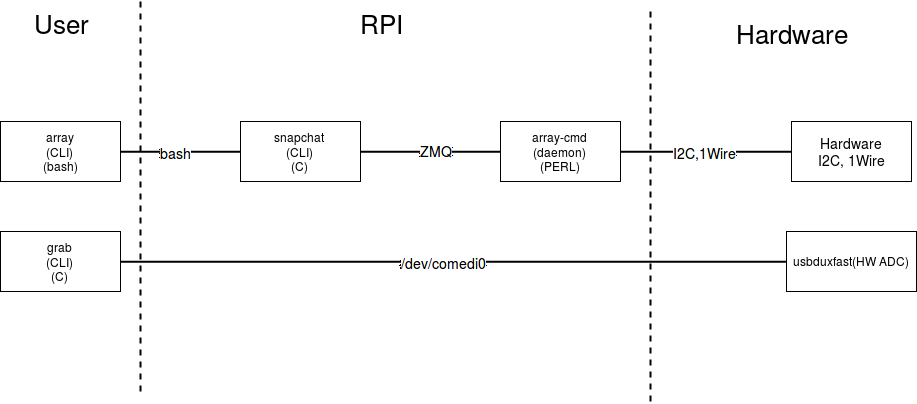
\includegraphics[width=\textwidth]{figures/mclurs_app1}
	\caption{MCLURS using Grab to do long or short recordings} \label{fig:mclurs:grab}
\end{figure}

\todo{described multibox-setup}
In figure \ref{fig:mclurs:snapshot}, \textit{array} also interacts with the system to set hardware properties. \textit{Snapshot} is used to capture from \textit{comedi0}, when a trigger-command is received from \textit{trig}.
Trig can either be instructed to talk to \textit{snapshot} directly, or to \textit{array-cmd}. If \textit{array-cmd} is chosen, metadata about hardware such as connected microphones, filters, recording box uuid, is saved.

\begin{figure}[h!]
	\centering
	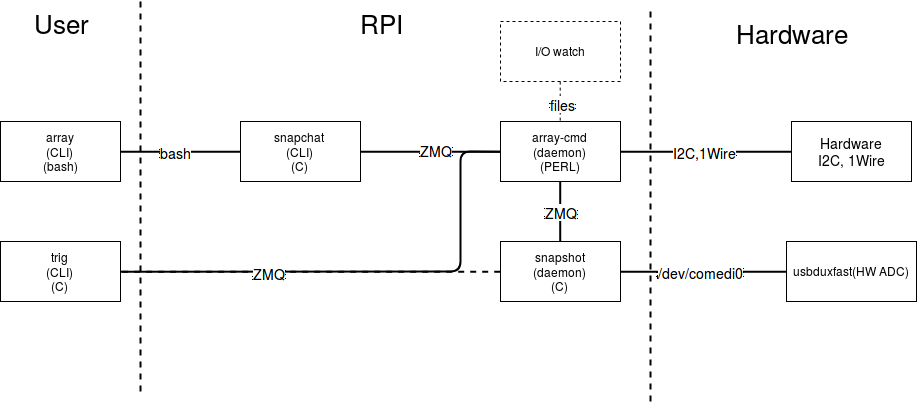
\includegraphics[width=\textwidth]{figures/mclurs_app2}
	\caption{MCLURS using snap to do long, short or trigger recordings. Iowatch has not been made, but was intended to to synchronize files to a remote destination} \label{fig:mclurs:snapshot}
\end{figure}
\todo{Fix lines around boxes in figures above.}

\subsubsection{Limitations} \label{sec:existingsystem:limitations}
MCLURS has some limitations that makes it difficult to make the system usable in all use cases.  \\

\textbf{Bandwidth}. In MCLURS the data is saved locally with recorded. Since the ADC produces worst-case 6 mb/sec of data, and the data is written to a local storage, a total of 16 MB/sek of bandwidh it consumed. If the data should also be streamed, this would require 18 MB/sec of bandwidth. Since MCLURS is running on a single RPI which suffers from Ethernet is attached to the USB-bus\todo{Cite}, it has been found by experiments\footnote{By Thor Andreassen}, that the USB-bus of the PI cannot transfer 18 MB/sec of data.\\

\textbf{Live processing}. As recordings are saved to files locally, it is not possible to process the files online. Some attempts have been to process data on the RPI, but with limited success, as the RPI is not very powerful compared to alternative hardware. \\

\textbf{Responsibility}. From a design perspective, the responsibility of a single RPI is not welldefined, as the RPI captures data from the ADC, saves the data to local storage, and possibly process the data. \\

\textbf{Backup}. As the data is stored on local storage, there is no backup of the data, in case the storage devices is lost. If copying of the data is attempted while recording, the USB-bus will be congested.

 
\subsubsection{Streaming Idea} \label{sec:streamingidea}
From the use cases and by looking into the \textit{Zebra Finch}\citep{larsen2016system} project, it became clear to split MCLURS's functionality into network attached nodes, in order to make MCLURS support online processing of recordings. If MCLURS's recording boxes are streaming the recordings instead of saving them locally, some of the limitations are eliminated and MCLURS allows for online audio processing. As in the \textit{Zebra Finch} project, a network attached device is then made responsible for saving streams, such that they can be replayed at a later time. This device will be referred to as \program{Historian}, as it saves streams with respect to time. The \textit{Zebra Finch} project implements the publisher/subscriber pattern in order to deliver the streams to multiple nodes by the use of multicast groups. \todo{Discuss limitations of new architecture in \textit{Discussion} section}
Chapter \ref{chp:analysis} elaborates on the idea of using streams.\\

The following figures show how the idea of streaming can be used in three types of recording.

Figure \ref{fig:idea:longrecording}, \ref{fig:idea:shortrecoring} and \ref{fig:idea:triggerrecording} show how long, short and trigger recordings respectively can be implemented with streams.

\missingfigure{Long recording}
\missingfigure{Short recording}
\missingfigure{Trigger recording}

\section{List of Achievements}
\todo{Describe what has been done in this project}
\begin{itemize}
	\item Analysis of use cases
	\item Find requirements
	\item Design architecture that fulfils requirements
	\item Make Proof-of-Concept implementation
	\item Verify requirements are fulfilled
\end{itemize}

\section{Conclusion}
\todo{Write sub-conclusion}
- conclude three types of recordings are used
- the system is used in different environments, in air, on ground, "in water".
